\documentclass[11pt,a4paper]{article}
\usepackage{amsmath}
\usepackage[margin=2cm]{geometry}
\usepackage{graphicx}
\usepackage{tikz}
\pagestyle{empty}
\usetikzlibrary{arrows.meta,positioning,fit,backgrounds,calc}

\definecolor{cInput}{RGB}{70,130,180}
\definecolor{cBase}{RGB}{42,157,143}
\definecolor{cCore}{RGB}{32,120,102}
\definecolor{cAdapter}{RGB}{224,122,95}
\definecolor{cOut}{RGB}{65,105,225}
\definecolor{cNote}{RGB}{250,250,245}

\tikzset{
  box/.style={draw, rounded corners=3pt, minimum height=9mm, align=center, font=\footnotesize, line width=0.8pt},
  inbox/.style={box, fill=cInput!12, draw=cInput},
  basebox/.style={box, fill=cBase!12, draw=cBase},
  corebox/.style={box, fill=cCore!12, draw=cCore},
  adbox/.style={box, fill=cAdapter!12, draw=cAdapter},
  outbox/.style={box, fill=cOut!12, draw=cOut},
  note/.style={draw, rounded corners=3pt, fill=cNote, font=\scriptsize, align=left},
  arr/.style={-Latex, line width=0.9pt}
}

\begin{document}
\begin{center}
\resizebox{\textwidth}{!}{%
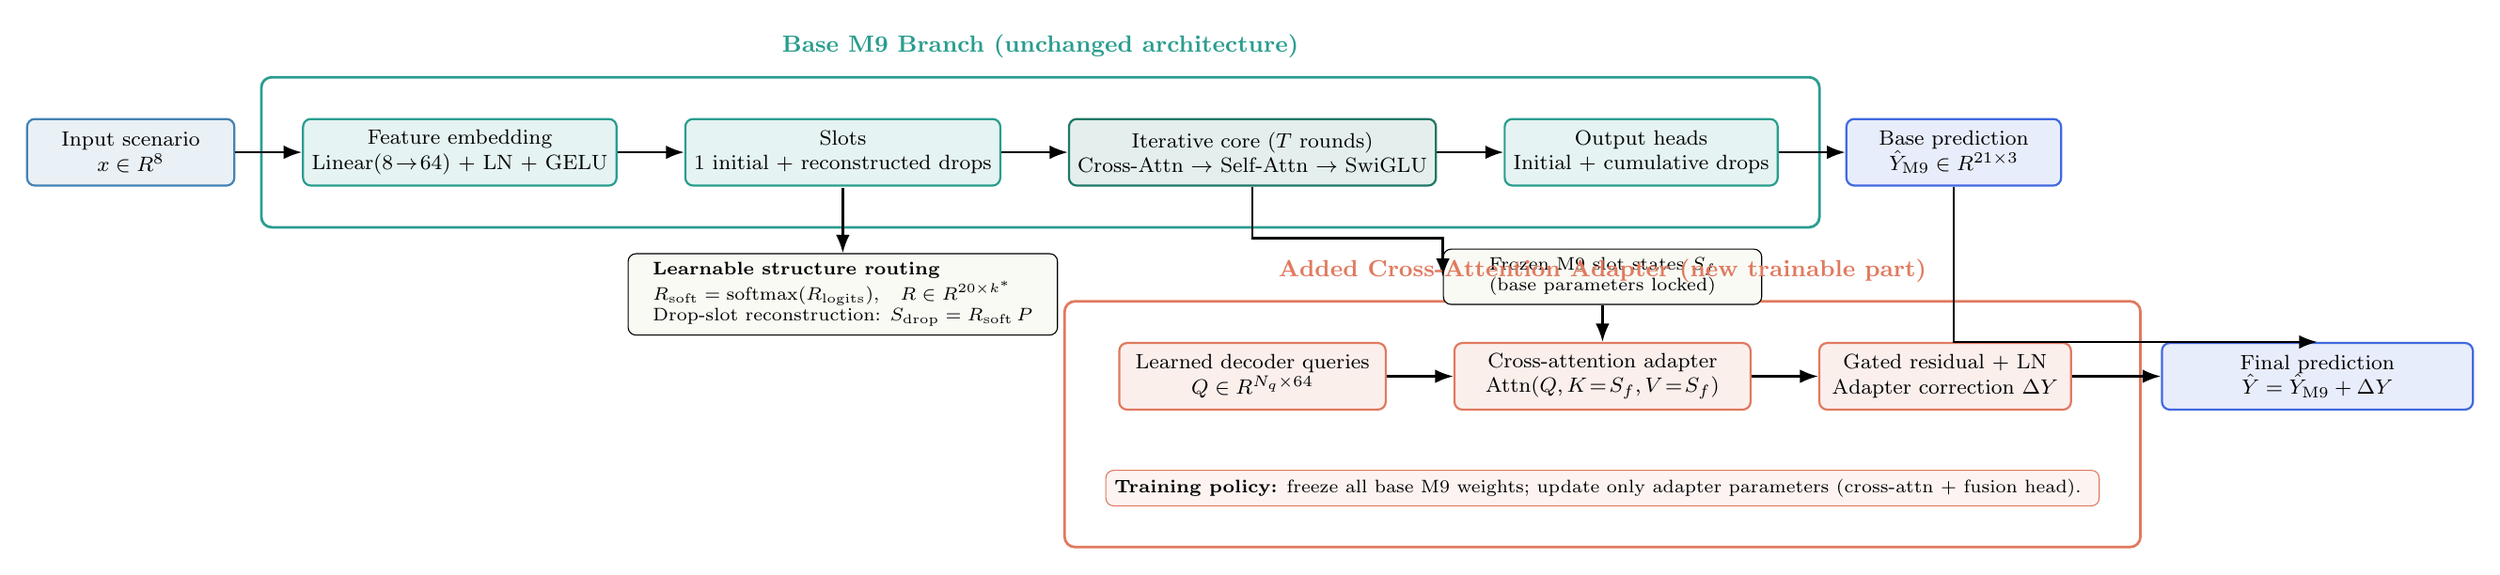
\begin{tikzpicture}[node distance=8mm and 9mm]

% ---------------- Main M9 branch ----------------
\node[inbox, minimum width=28mm] (x) {Input scenario\\$x\in\mathbb{R}^{8}$};
\node[basebox, minimum width=34mm, right=of x] (embed) {Feature embedding\\Linear$(8\!\to\!64)$ + LN + GELU};
\node[basebox, minimum width=33mm, right=of embed] (slots) {Slots\\1 initial + reconstructed drops};
\node[corebox, minimum width=40mm, right=of slots] (iter) {Iterative core ($T$ rounds)\\Cross-Attn $\to$ Self-Attn $\to$ SwiGLU};
\node[basebox, minimum width=33mm, right=of iter] (head) {Output heads\\Initial + cumulative drops};
\node[outbox, minimum width=29mm, right=of head] (yhat) {Base prediction\\$\hat{Y}_{\text{M9}}\in\mathbb{R}^{21\times3}$};

\draw[arr] (x) -- (embed);
\draw[arr] (embed) -- (slots);
\draw[arr] (slots) -- (iter);
\draw[arr] (iter) -- (head);
\draw[arr] (head) -- (yhat);

% Relation matrix details under slot block
\node[note, below=9mm of slots, minimum width=58mm] (rel) {
\textbf{Learnable structure routing}\\
$R_{\text{soft}}=\mathrm{softmax}(R_{\text{logits}})$,\quad $R\in\mathbb{R}^{20\times k^*}$\\
Drop-slot reconstruction: $S_{\text{drop}}=R_{\text{soft}}\,P$
};
\draw[arr] ($(slots.south)+(0,-0.2mm)$) -- (rel.north);

% ---------------- Adapter branch ----------------
\node[adbox, minimum width=36mm, below=21mm of iter] (q) {Learned decoder queries\\$Q\in\mathbb{R}^{N_q\times64}$};
\node[adbox, minimum width=40mm, right=of q] (xca) {Cross-attention adapter\\$\mathrm{Attn}(Q, K\!=\!S_f, V\!=\!S_f)$};
\node[adbox, minimum width=34mm, right=of xca] (fuse) {Gated residual + LN\\Adapter correction $\Delta Y$};

\draw[arr] (q) -- (xca);
\draw[arr] (xca) -- (fuse);

% frozen slot states feeding adapter K/V
\node[note, above=5mm of xca, minimum width=43mm] (frozen) {Frozen M9 slot states $S_f$\\(base parameters locked)};
\draw[arr] (iter.south) -- ++(0,-7mm) -| (frozen.west);
\draw[arr] (frozen.south) -- (xca.north);

% Final composition
\node[outbox, minimum width=42mm, right=12mm of fuse] (final) {Final prediction\\$\hat{Y}=\hat{Y}_{\text{M9}} + \Delta Y$};
\draw[arr] (fuse) -- (final);
\draw[arr] (yhat.south) |- (final.north);

% Training scope banner
\node[note, draw=cAdapter, fill=cAdapter!8, below=8mm of xca, minimum width=96mm] (train) {
\textbf{Training policy:} freeze all base M9 weights; update only adapter parameters (cross-attn + fusion head).
};

% Global groups
\begin{scope}[on background layer]
  \node[draw=cBase, rounded corners=4pt, line width=1.0pt, fit=(embed)(slots)(iter)(head), inner sep=5.5mm] (gbase) {};
  \node[draw=cAdapter, rounded corners=4pt, line width=1.0pt, fit=(q)(xca)(fuse)(train), inner sep=5.5mm] (gadapt) {};
\end{scope}

\node[font=\bfseries\small, text=cBase] at ($(gbase.north)+(0,4mm)$) {Base M9 Branch (unchanged architecture)};
\node[font=\bfseries\small, text=cAdapter] at ($(gadapt.north)+(0,4mm)$) {Added Cross-Attention Adapter (new trainable part)};

\end{tikzpicture}
}
\end{center}
\end{document}
